\chapter{Evaluation} \label{C:evaluation}
The section covers the evaluation of the Kihi Runner. Specifically, this section analyses the results of the aforementioned benchmark suites on the final version of the Kihi Runner. It begins with an analysis of the micro benchmarks which examine the individual elements of the Kihi Runner. This is followed by the macro benchmarks which examine the performance of these optimisations against a small set of representative benchmark programs.

\section{Method}
All these benchmarks and graphs were autogenerated by the benchmark suite. The instructions for reproducing these benchmarks are provided in the project's readme which can be found on Gitlab. These specific benchmarks were run on a computer with an i5-4670K CPU @ 3.40GHZ and 8GB of 2400MHZ RAM.

\section{Micro Benchmarks}
This section includes benchmarks on compilation time and operator evaluation. The compilation time analysis looks at how optimisation level and program length affect compilation time. The operator evaluation analysis looks at how operators handle abstractions of varying length and successive applications. The latter is essentially a test of the effectiveness of the optimised representation. These benchmarks are executor agnostic as there is no need to find an operator when the program consists of only one operator.

\subsection{Compilation vs Program Length}
\begin{figure}[H]
    \centering
    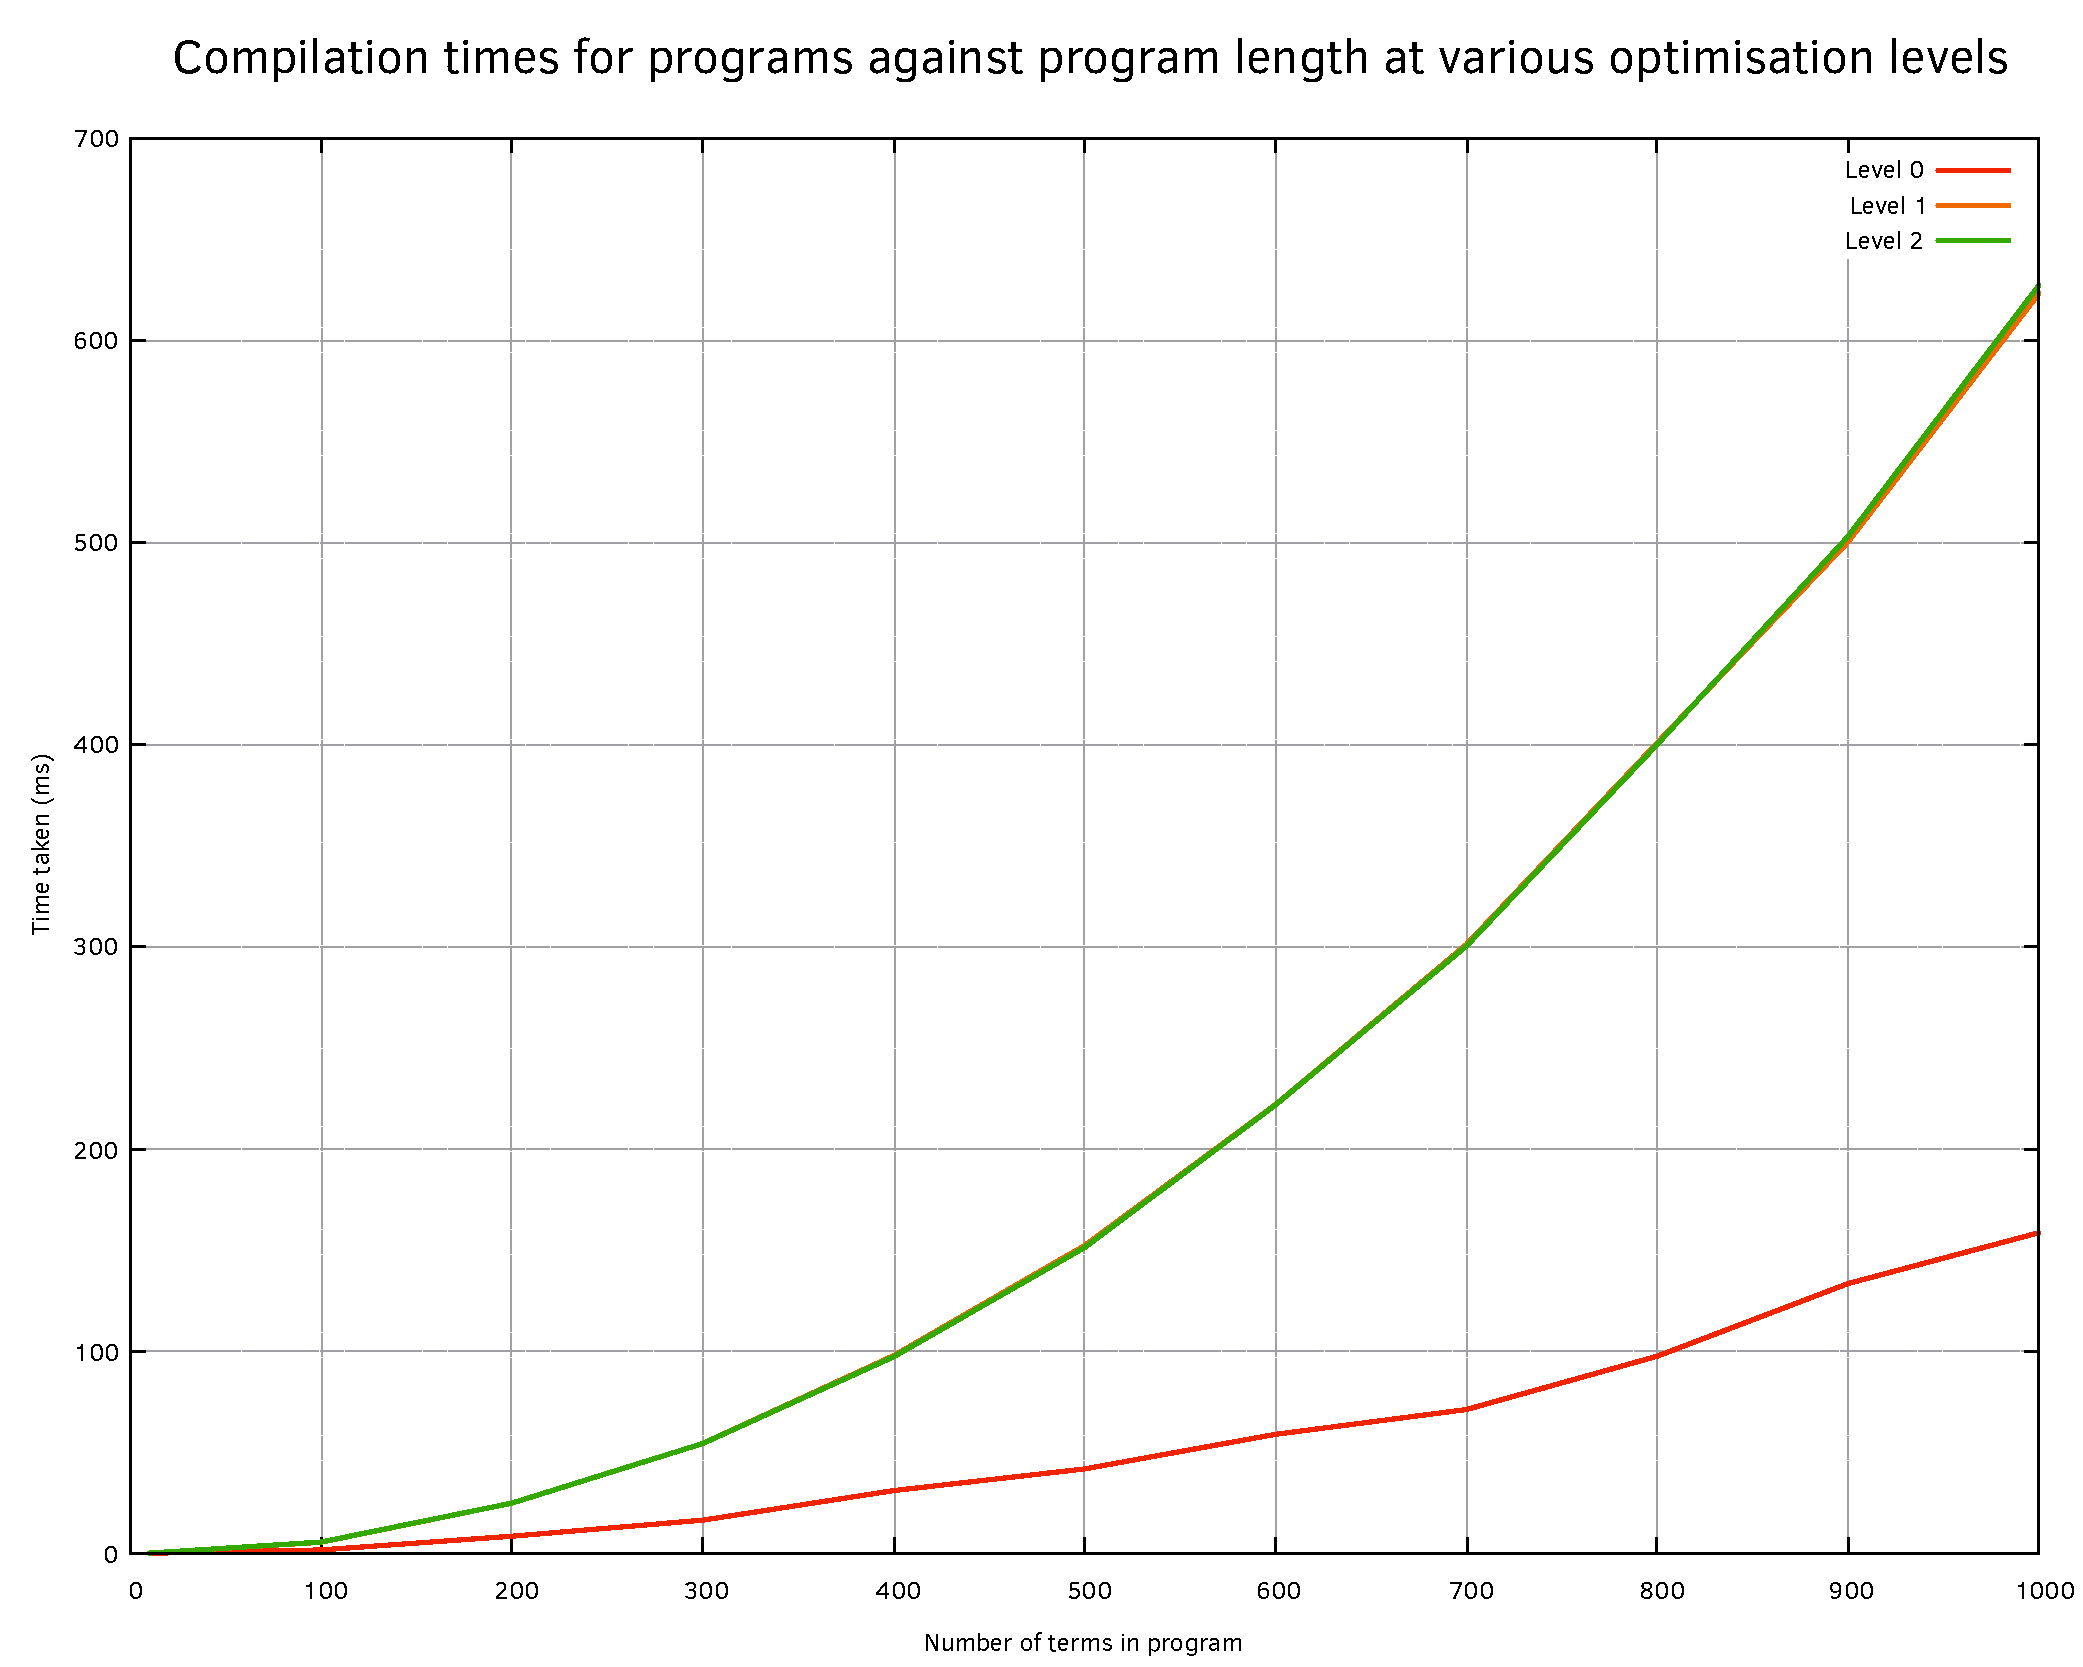
\includegraphics[width=\textwidth - 100pt]{04_results/images/compilation_results}

    \begin{center}
    \begin{tabular}{ |c|c|c|c|c| } 
    \hline
    Program & Program Length & Level 0 & Level 1 & Level 2 \\ 
    \hline
    delve & 10 & 14.365 us & 55.416 us & 60.233 us\\
    \hline
    delve & 100 & 1.6734 ms & 5.4487 ms & 5.5868 ms\\
    \hline
    delve & 200 & 8.3995 ms & 24.780 ms & 24.802 ms\\
    \hline
    delve & 300 & 16.349 ms	& 54.290 ms& 54.245 ms\\
    \hline
    delve & 400 & 30.992 ms & 97.726 ms & 	97.198 ms\\
    \hline
    delve & 500 & 41.730 ms &152.20 ms & 151.23 ms \\
    \hline
    delve & 600 & 58.856 ms &221.79 ms & 221.72 ms \\
    \hline
    delve & 700 & 71.066 ms &300.98 ms & 300.28 ms \\
    \hline
    delve & 800 & 97.426 ms &400.76 ms & 399.97 ms \\
    \hline
    delve & 900 & 133.36 ms &500.20 ms & 502.94 ms \\
    \hline
    delve & 1000 & 158.58 ms & 623.05 ms & 627.05 ms \\
    \hline
    \end{tabular}
    \end{center}
    \caption{Program length vs compilation time at various optimisation levels.}
    \label{fig:compilation_results}
\end{figure}

Compilation consists of up to three stages: parsing, symbol detection, and symbol optimisation. The optimisation level determines the number of stages in the compilation. Optimisation level 0 only includes parsing, whilst level 2 includes all three. The results in figure \ref{fig:compilation_results} illustrate how compilation time changes as program length increases for varying optimisation levels. The results show that whilst level 0 scales approximately linearly with program length, level 1 and 2 scale superlinearly. Interestingly however, optimisation level 2 incurs almost no additional cost over just level 1.

The linear behaviour of level 0 is unsurprising because the parser is a simple linear algorithm that simply performs a single pass through the source code. However, the superlinear behaviour of level 1 is surprising because the symbol detection algorithm is also linear. This is most likely due to the memory allocation and initialisation that potentially happens on each term. As the program grows larger the size of the memory allocation increases in tandem with the frequency of memory allocations resulting in $\theta(n^2)$ complexity. The negligible cost of symbol optimisation is also surprising, and can be attributed to the small number and size of symbols that need to be optimised. In the case of this program, there are only eight symbols with at most six terms regardless of program length due to repetition. Since the symbol optimisation algorithm scales linearly with symbol size and symbol count it becomes negligible as the program size increases.

\subsection{Operators}
\subsubsection{Operator vs Abstraction Length}
\begin{figure}[H]
    \centering
    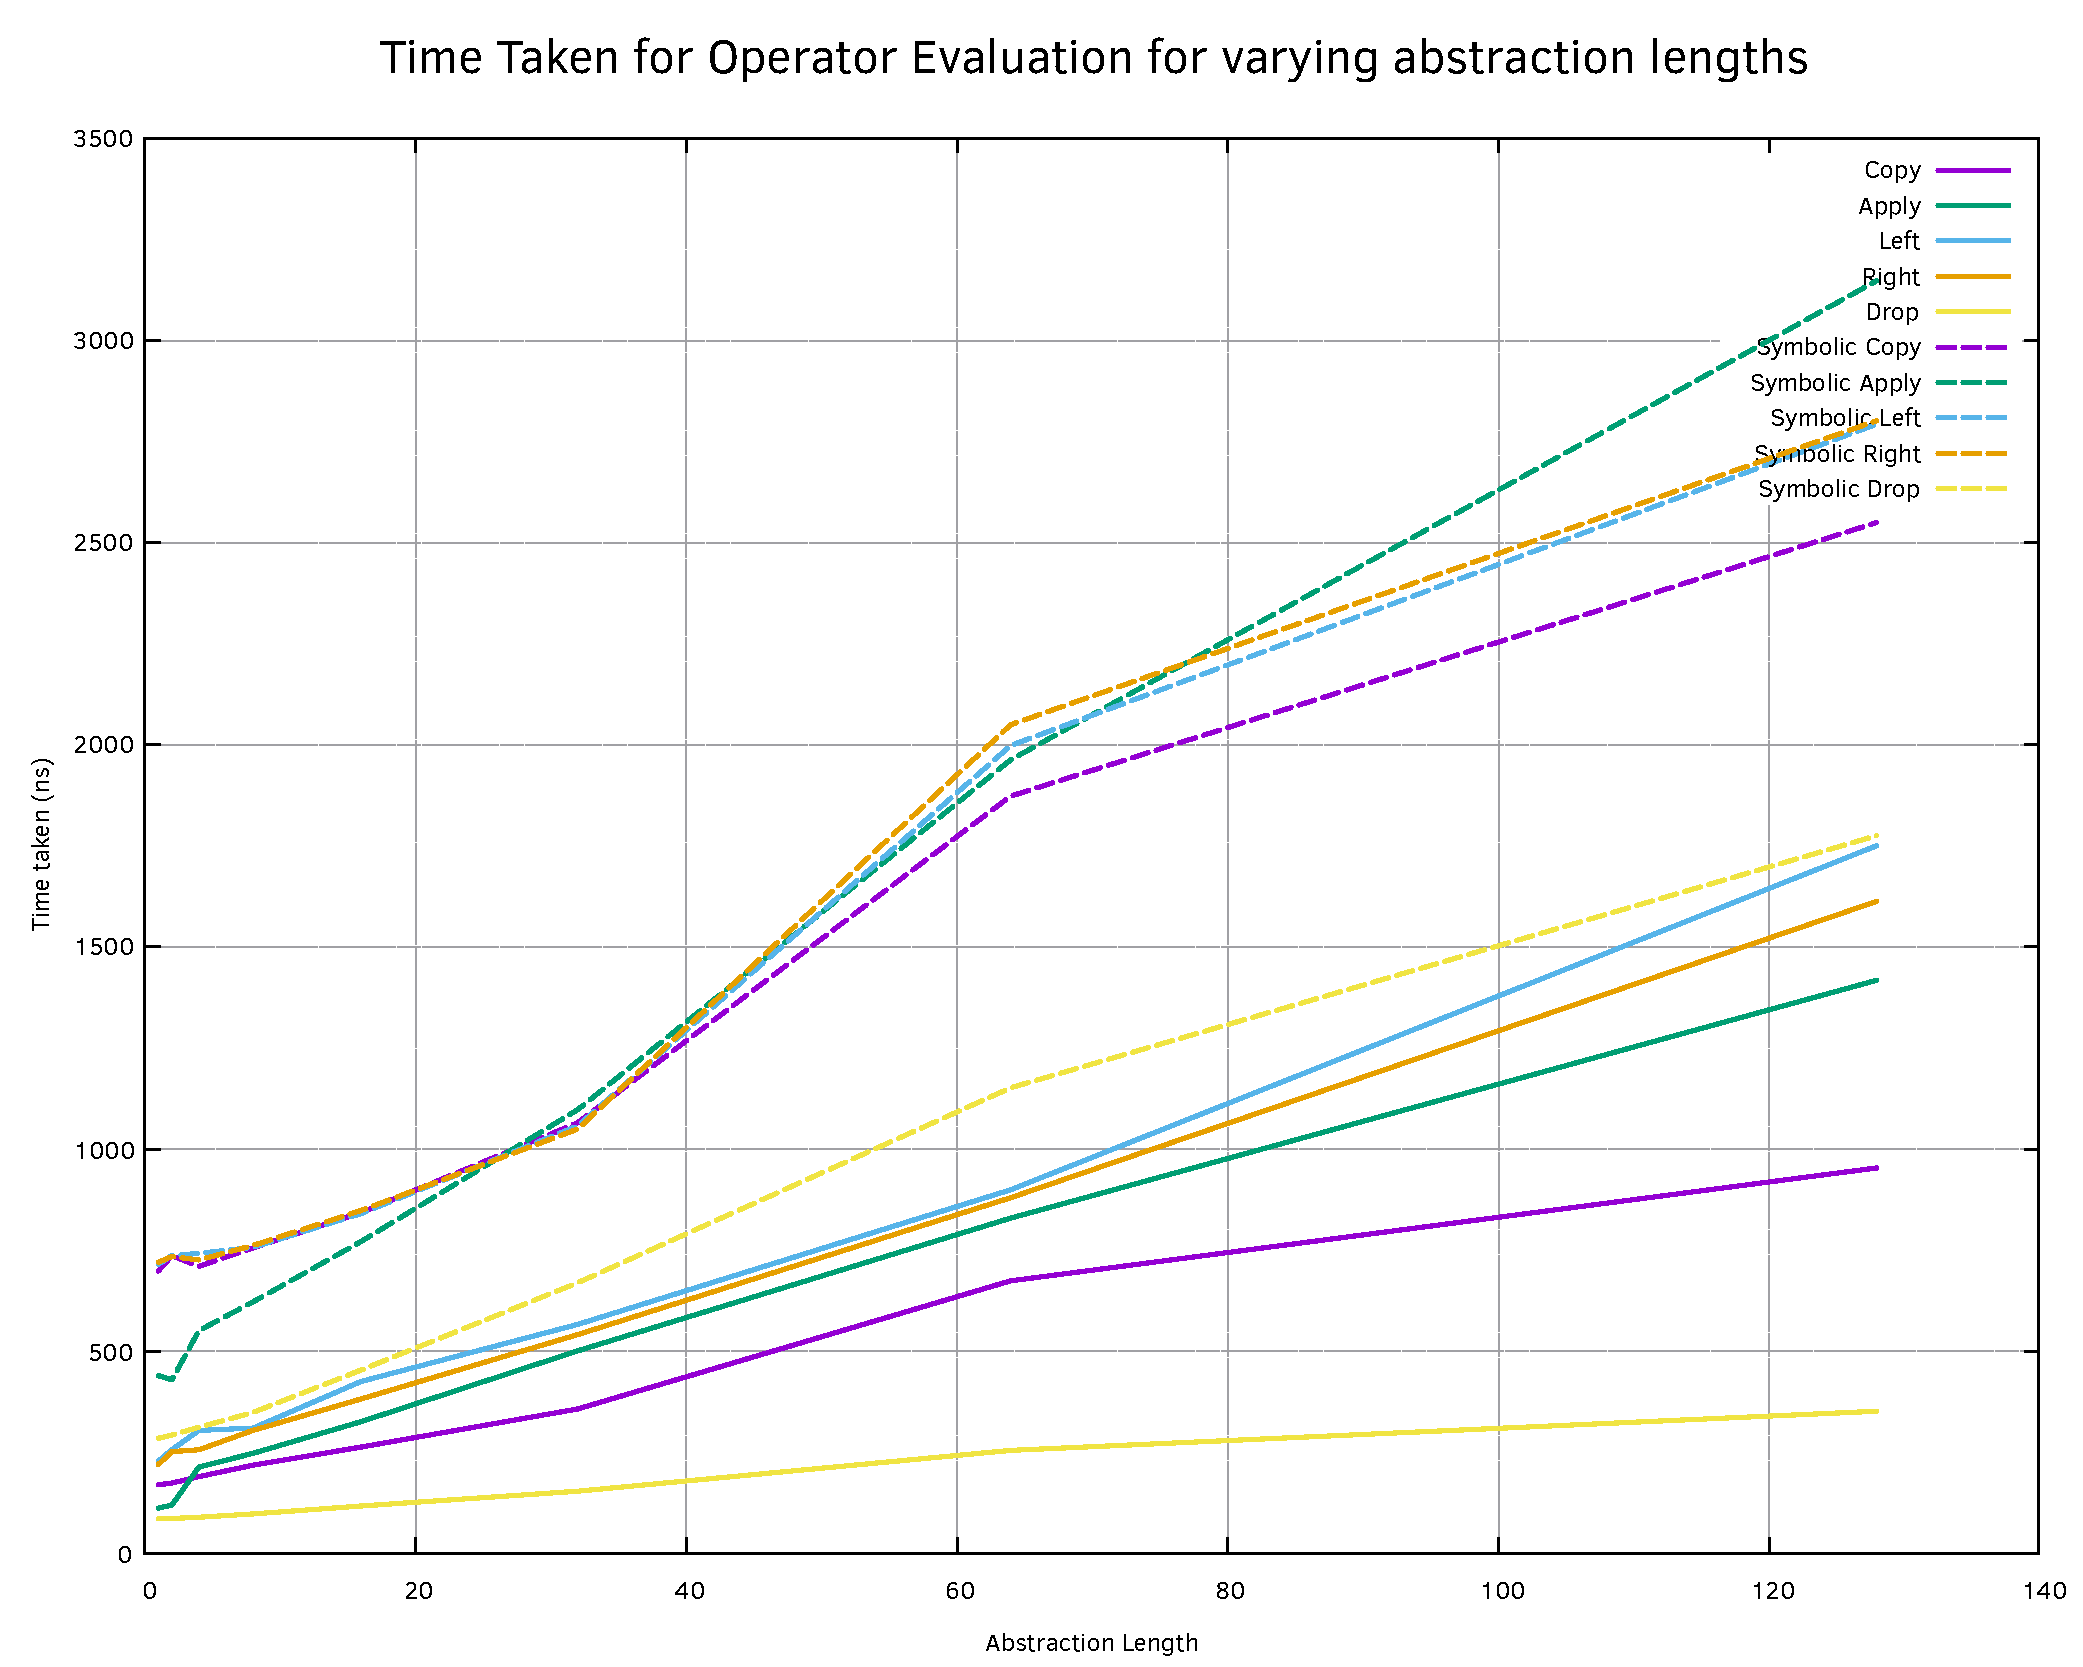
\includegraphics[width=\textwidth - 100pt]{04_results/images/basic_operator_results_2}

    \begin{center}
    \begin{tabular}{ |c|c|c|c|c|c| } 
    \hline
    Abstraction Length & Copy & Apply & Left & Right & Drop \\
    \hline
    1 & 169.48 ns& 111.97 ns & 227.83 ns & 219.19 ns & 84.786 ns \\
    \hline
    2 & 173.73 ns& 118.98 ns & 255.91 ns & 251.56 ns & 85.886 ns \\
    \hline
    4 & 189.41 ns& 213.45 ns & 303.67 ns & 255.97 ns & 89.071 ns \\
    \hline
    8 & 217.64 ns& 247.26 ns & 309.54 ns & 303.68 ns & 97.224 ns \\
    \hline
    16 & 262.71 ns& 325.29 ns & 424.90 ns & 381.71 ns & 117.02 ns \\
    \hline
    32 & 356.94 ns& 500.84 ns & 566.31 ns & 540.59 ns & 153.60 ns \\
    \hline
    64 & 673.85 ns& 829.02 ns & 898.72 ns & 879.33 ns & 254.49 ns \\
    \hline
    128 & 952.81 ns& 1416.8 ns & 1749.8 ns & 1612.3 ns & 351.46 ns \\
    \hline
    \end{tabular}
    \end{center}
    \caption{Time taken for operator evaluation with varying abstraction lengths.}

    \begin{center}
    \begin{tabular}{ |c|c|c|c|c|c| } 
    \hline
    Abstraction Length & Copy & Apply & Left & Right & Drop \\
    \hline
    1 & 698.05 ns & 439.56 ns & 715.05 ns & 719.63 ns & 284.33 ns \\
    \hline
    2 & 736.09 ns & 429.20 ns & 735.88 ns & 734.22 ns & 292.42 ns \\
    \hline
    4 & 709.83 ns & 550.59 ns & 741.79 ns & 725.09 ns & 311.68 ns \\
    \hline
    8 & 755.02 ns & 621.54 ns & 756.69 ns & 761.26 ns & 348.12 ns \\
    \hline
    16 & 842.81 ns & 771.26 ns & 839.91 ns & 847.95 ns & 453.46 ns \\
    \hline
    32 & 1064.7 ns & 1097.1 ns & 1056.8 ns & 1049.4 ns & 669.16 ns \\
    \hline
    64 & 1872.2 ns & 1961.9 ns & 1997.4 ns & 2049.2 ns & 1151.3 ns \\
    \hline
    128 & 2549.2 ns & 3147.3 ns & 2792.4 ns & 2800.8 ns & 1774.9 ns \\
    \hline
    \end{tabular}
    \end{center}
    \caption{Time taken for symbolic operator evaluation with varying abstraction lengths.}
    \label{fig:basic_operator_results}
\end{figure}

Figure \ref{fig:basic_operator_results} shows the performance of the standard and symbolic operators on abstractions of varying length. A symbolic operator is an operator that has been converted into a symbol and optimised. The results show that all operators appear to scale linearly with abstraction size. This is unsurprising, as the most expensive aspects of operator evaluation are memory allocation and initialisation, both operations that scale linearly with the size of the abstraction. The results also show that symbolic optimisation is not a cost-free optimisation. There is a fixed overhead to utilising the optimised representation. However, the performance of the optimised representation degrades at approximately the same rate as the unoptimised version. This overhead is likely due to the machinery required to shift from standard execution to optimised execution. Specifically, the process of gathering abstractions for the optimised representation requires a non-negligible amount of work.

\subsubsection{Repeated Operator Application}
\begin{figure}[H]
    \centering
    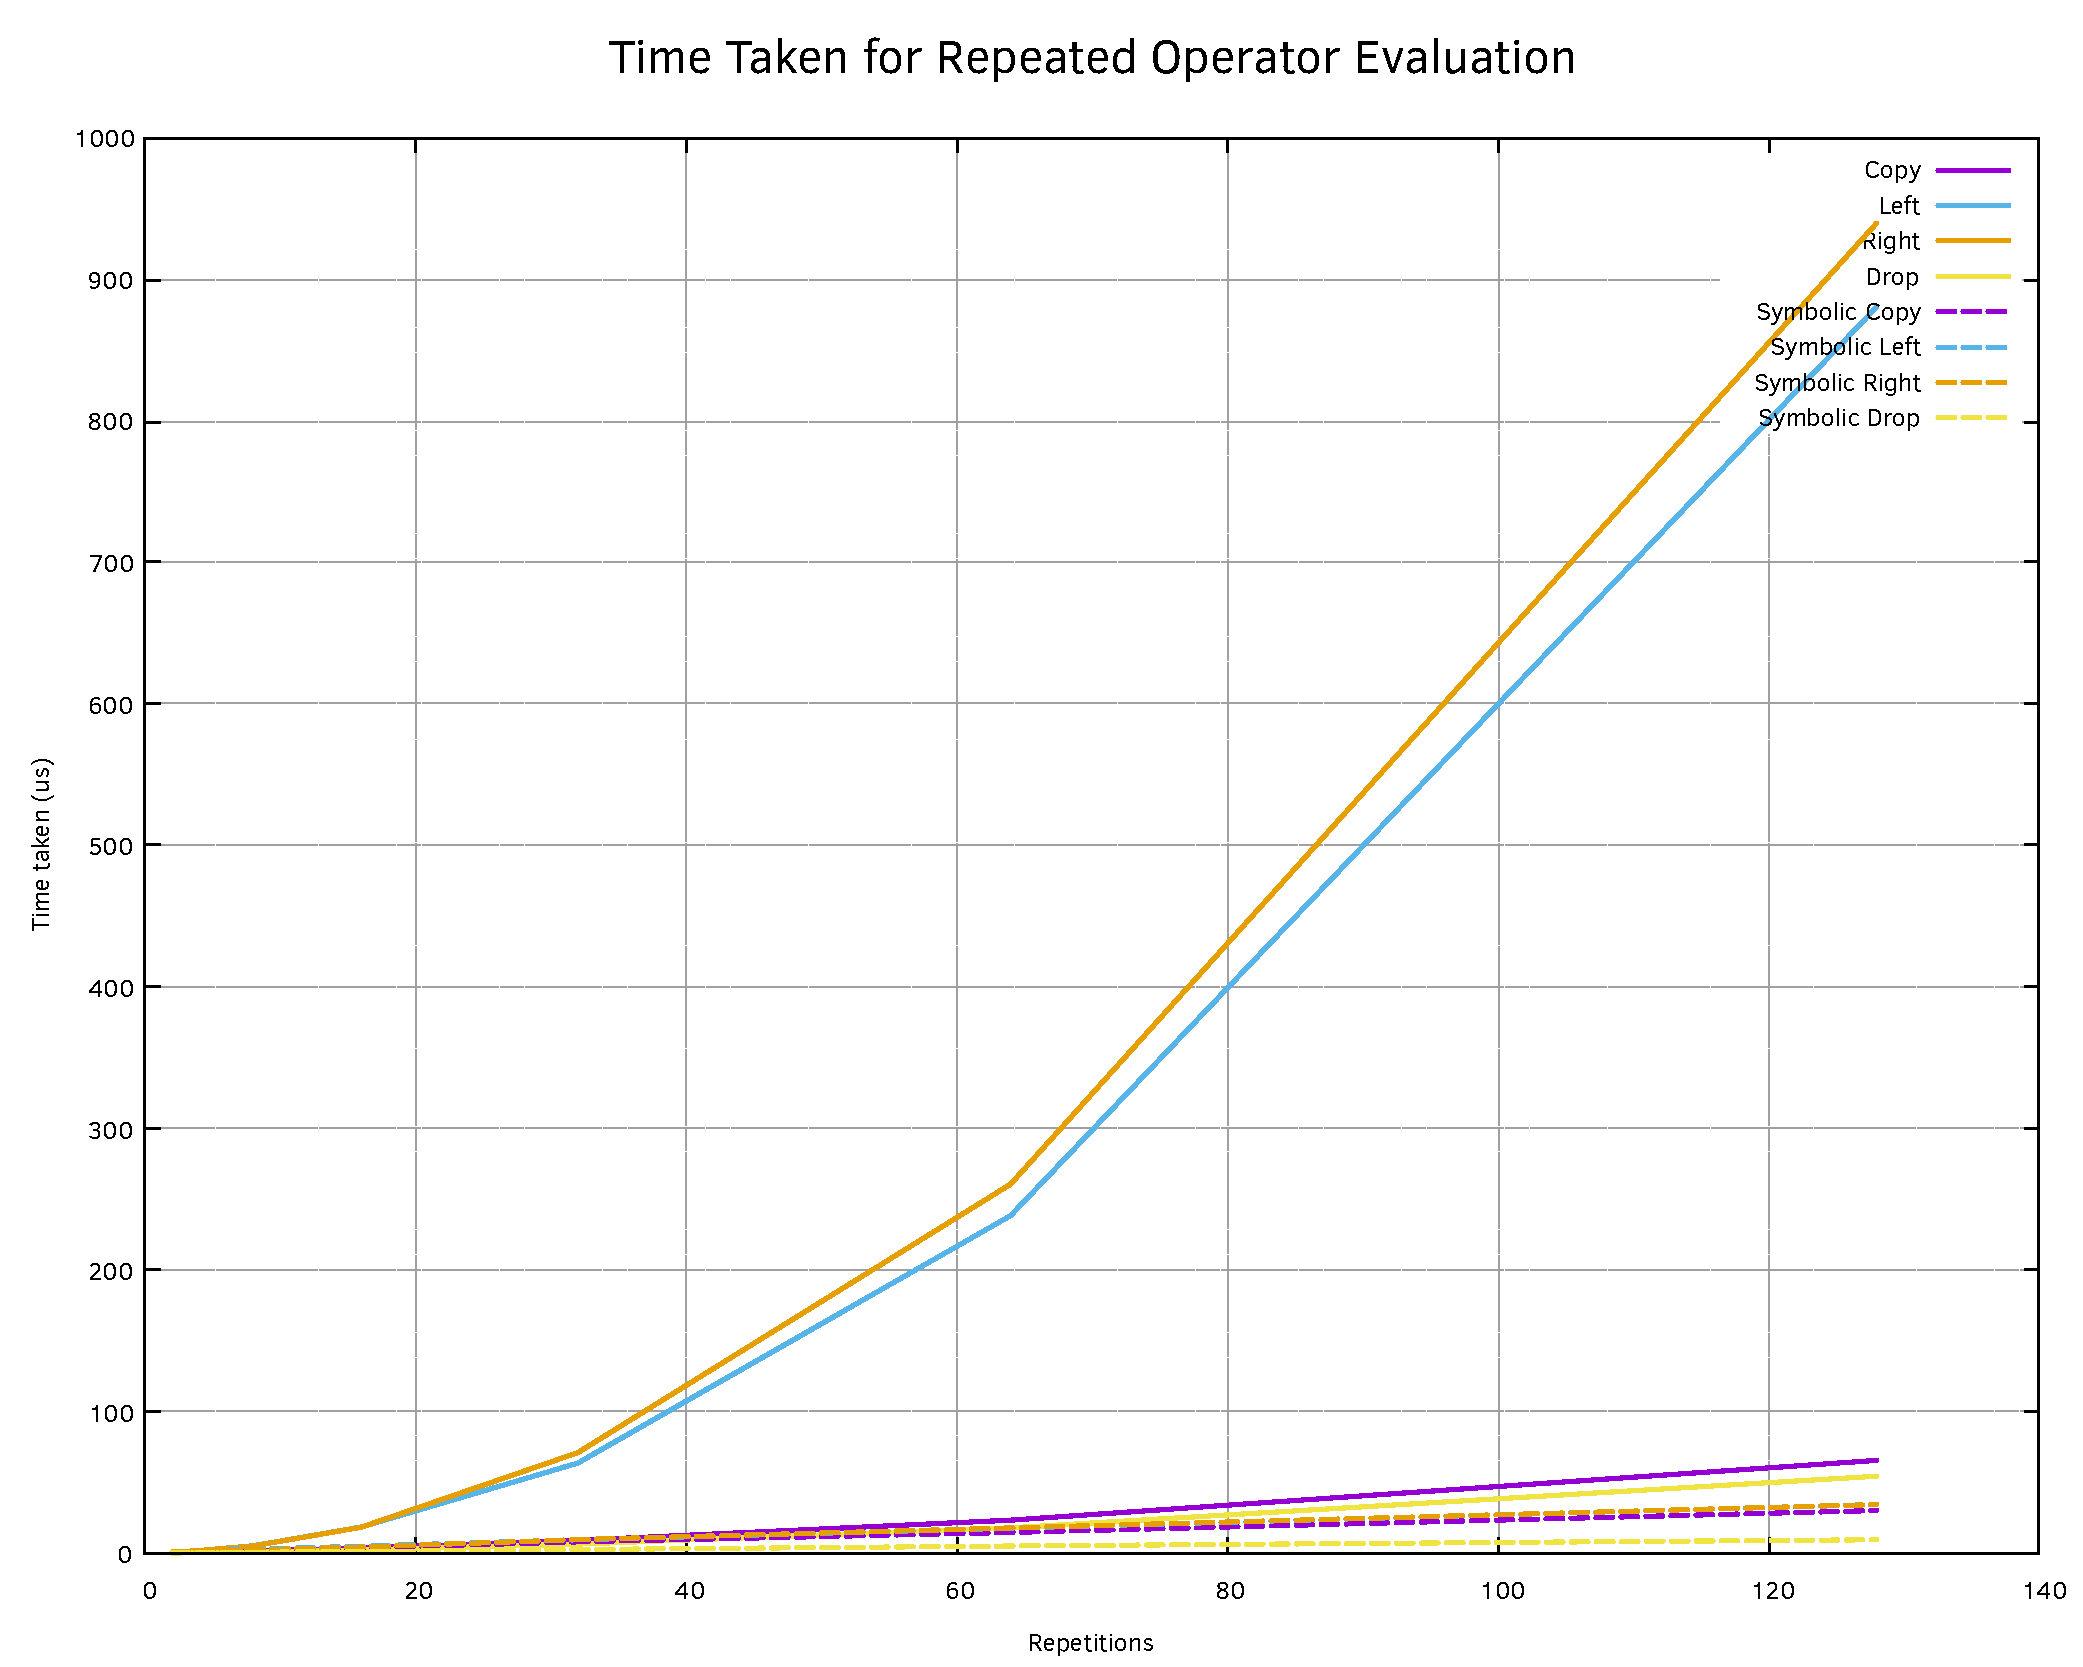
\includegraphics[width=\textwidth]{04_results/images/repeated_operator_results}

    \begin{center}
    \begin{tabular}{ |c|c|c|c|c|c| } 
    \hline
    Repetitions	& Copy & Left & Right & Drop \\
    \hline
    2 & 0.4419 us & 0.7791 us & 0.7384 us & 0.2061 us \\
    \hline
    4 & 0.8264 us & 1.9235 us & 1.8607 us & 0.3844 us \\
    \hline
    8 & 1.7557 us & 5.3294 us & 5.1021 us & 0.9550 us \\
    \hline
    16 & 3.7157 us & 18.537 us & 18.414 us & 2.4040 us \\
    \hline
    32 & 9.0936 us & 63.749 us & 71.145 us & 6.4837 us \\
    \hline
    64 & 23.417 us & 238.53 us & 260.82 us & 17.955 us \\
    \hline
    128 & 65.677 us & 880.67 us & 939.85 us & 54.382 us \\
    \hline
    \end{tabular}
    \end{center}
    \caption{Time taken for repeated operator evaluation.}

    \begin{center}
    \begin{tabular}{ |c|c|c|c|c|c| } 
    \hline
    Repetitions	& Copy & Left & Right & Drop \\
    \hline
    2 & 1.0827 us & 1.0302 us & 1.0807 us & 0.4705 us \\
    \hline
    4 & 1.4615 us & 1.6106 us & 1.5678 us & 0.5493 us \\
    \hline
    8 & 2.2003 us & 2.7681 us & 2.4266 us & 0.7250 us \\
    \hline
    16 & 3.8366 us & 5.0191 us & 4.3835 us & 1.1549 us \\
    \hline
    32 & 8.0420 us & 9.5310 us & 9.7107 us & 2.6130 us \\
    \hline
    64 & 14.749 us & 17.855 us & 17.940 us & 5.1694 us \\
    \hline
    128 & 30.267 us & 34.555 us & 34.524 us & 9.6662 us \\
    \hline
    \end{tabular}
    \end{center}
    \caption{Time taken for repeated symbolic operator evaluation.}
    \label{fig:repeated_operator_results}
\end{figure}

Figure \ref{fig:repeated_operator_results} shows that for repeated applications of left and right, the optimised encodings have substantially better performance. In contrast to the non-optimised versions which display exponentially worsening performance, the optimised versions appear to scale linearly. This significant performance boost is likely due to the optimised representation's ability to evaluate the entire series of operators in one find and replace scan. This stands in contrast to the unoptimised representation which must repeatedly manipulate the system's state.

\section{Macro Benchmarks}
This section provides benchmarks of the Kihi Runner on real Kihi programs. This section first describes the programs being used as benchmarks, and establishes why they are appropriate. 

\subsection{Benchmark Programs}
An effort has been made to ensure the benchmark programs are representative of typical Kihi programs, but this is difficult because Kihi is not an ordinary programming language. However, what has been attempted is finding programs with a variety of operator distributions and structures in order to provide good coverage of the potential program space. Structures here referring to the encodings, such as church numerals, used in the program. This led to the choice of three main benchmark programs:

\begin{figure}[H]
\centering
\begin{enumerate}
    \item \textbf{Count}; Outputs all the natural numbers (as church numerals) in order.
    \item \textbf{Count\_Bind}; Outputs all the natural numbers (as church numerals) in order using a bind stucture \cite{jones2018practice}.
    \item \textbf{Count\_List}; Outputs all the natural numbers (as church numerals) in order using a list stucture \cite{jones2018practice}.
\end{enumerate}
\end{figure}

The instruction distributions of these programs are shown in figure \ref{fig:program_term_distribution}. The distribution shown provides decent coverage of the variety of terms, and potential distributions. Apply is necessarily common because it is the only mechanism that can extend the length of the program.

\begin{figure}[hb]
    \centering
    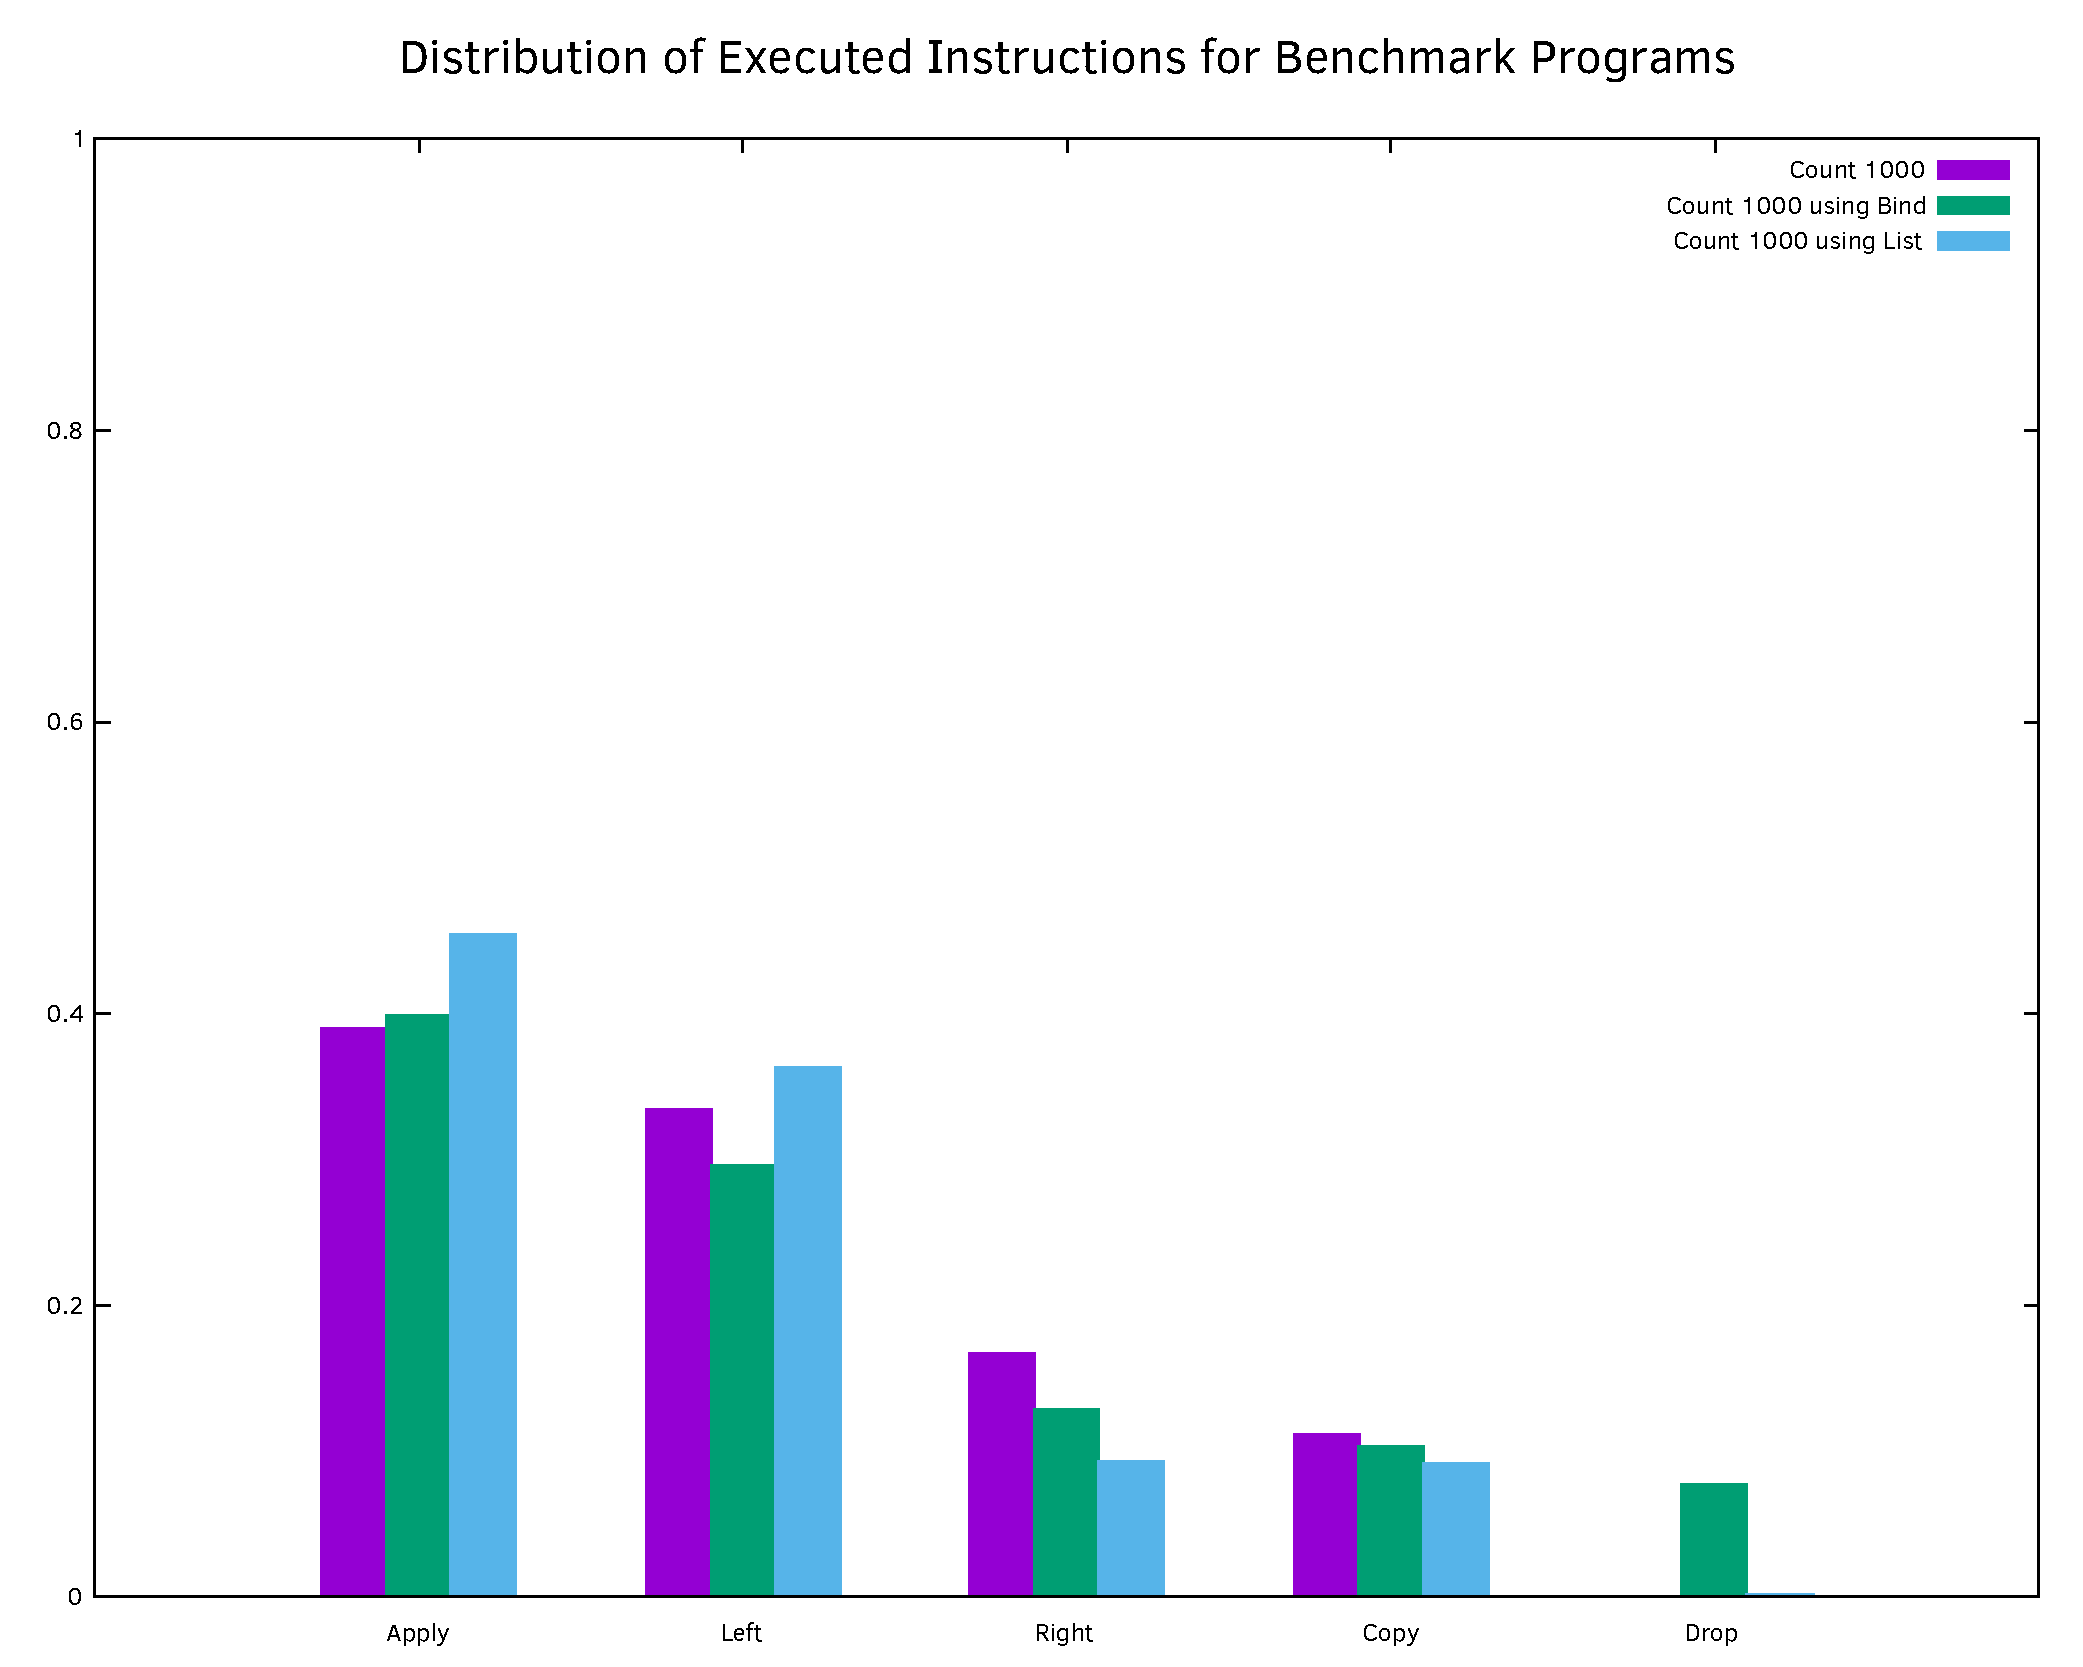
\includegraphics[width=\textwidth]{04_results/images/program_term_distribution}
    \caption{Chart of operator distributions for the benchmark programs.}
    \label{fig:program_term_distribution}
\end{figure}


\subsection{Analysis}
Figures \ref{fig:reduce_count_performance} to \ref{fig:reduce_count_list_performance} demonstrate the reduce executors performance on the various count programs at varying optimisation levels. These figures show that optimisation level 1 provides a significant boost to Kihi Runner's performance in general across all programs. This stands in contrast to optimisation level 2 which only provides a slight improvement to performance on `count' and `count\_list', and provides no noticeable improvement to `count\_bind'. This suggests that the optimisation algorithm is unable to effectively decode the structure underlying `count\_bind'.

Figures \ref{fig:reduce_count_efficiency} to \ref{fig:reduce_count_list_efficiency} demonstrate the efficiency of the reduce executor at various optimisation levels. Perhaps surprisingly, optimisation level 1 increases the number of instructions that must be executed in order to compute the same number of outputs. This is due to the additional symbol expansion step required in order to process a symbol. Symbol expansion simply refers to the process of replacing a symbol with its corresponding terms. However, at optimisation level 2, the number of instructions decreases below level 0. This is because level 2 introduces the ability to execute symbols directly by utilising the find and replace algorithm. This not only removes the need for symbol expansion but also potentially captures multiple terms into a single execution step.

Overall, these figures suggest that the major performance gains are due to more efficient handling of memory. The fact that optimisation level 1, which replaces sequences of terms with an equivalent symbol, provides the majority of the performance boost strongly suggests that minimising the size and frequency of memory allocations and manipulations provides the greatest performance benefits. 

\begin{figure}[htb]
    \centering
    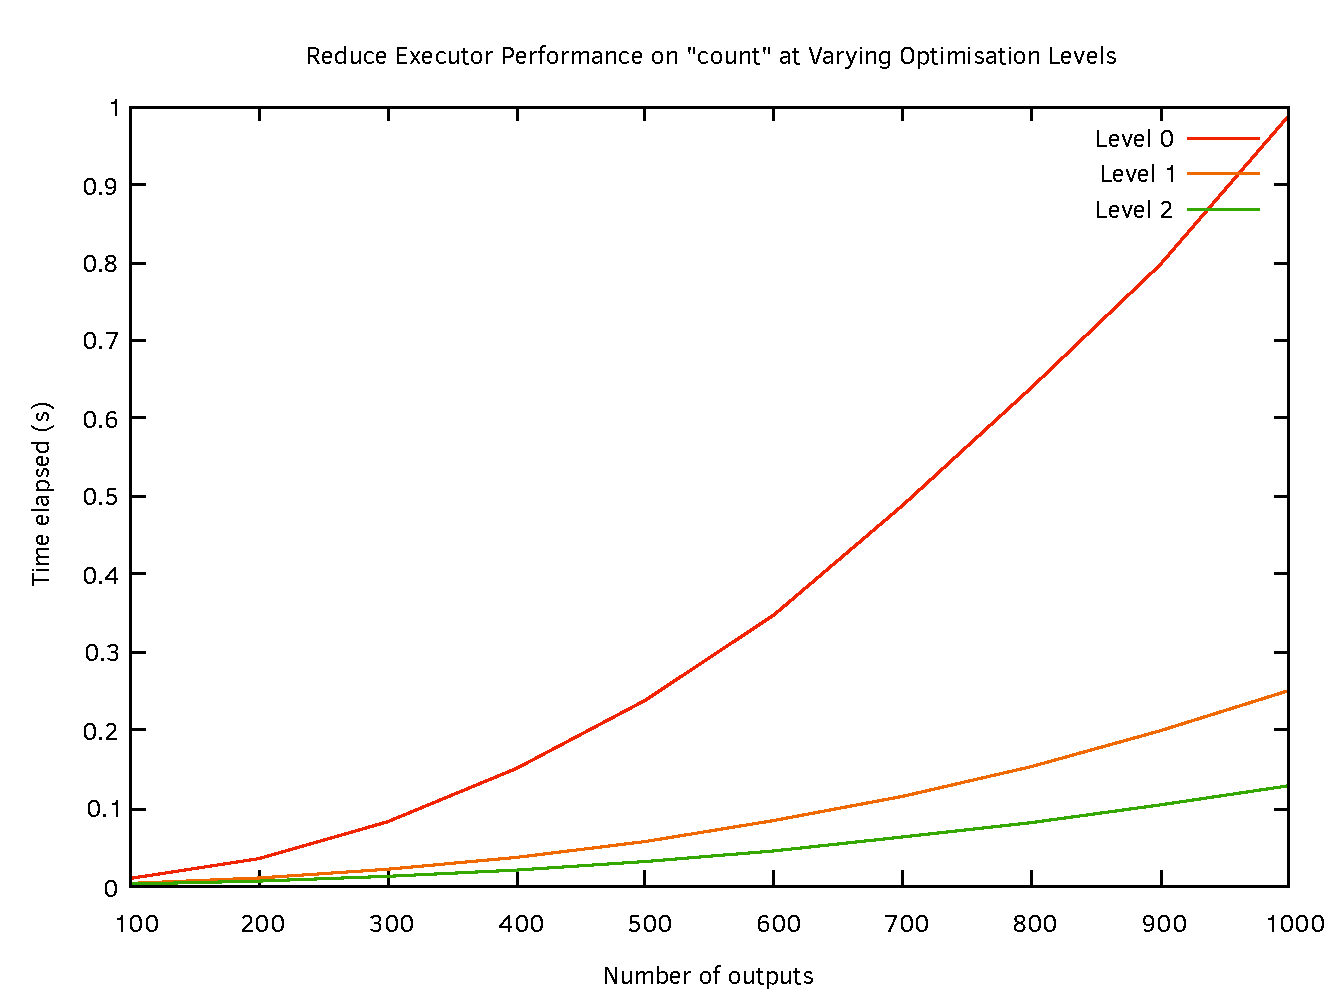
\includegraphics[width=\textwidth]{reduce_executor_fig_1}
    \caption{A chart demonstrating the effect of varying optimisations}
    \label{fig:reduce_executor_performance_on_count}
\end{figure}

\begin{figure}[htb]
    \centering
    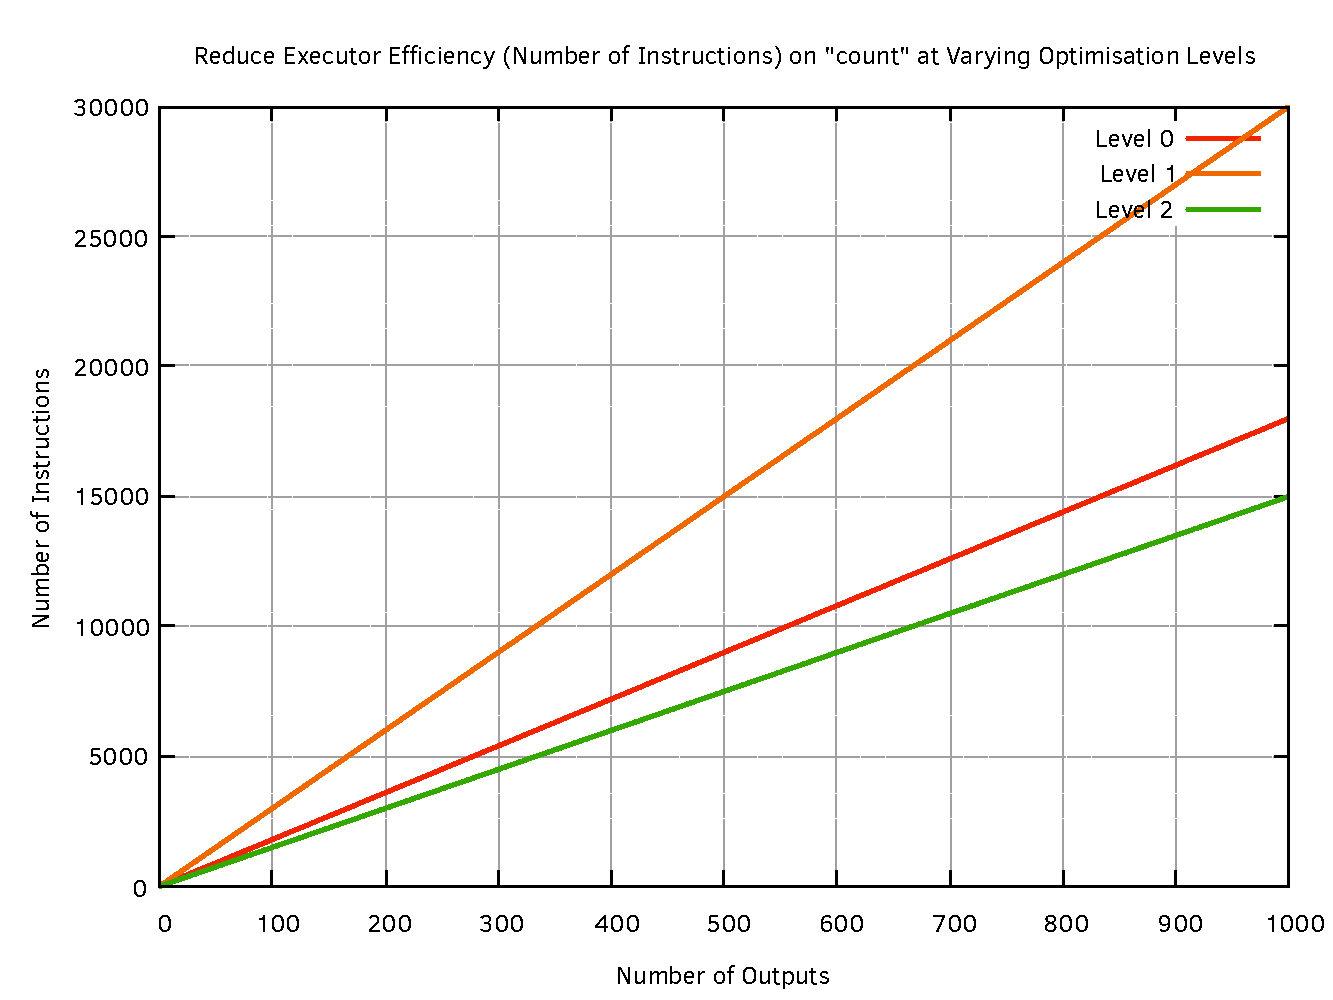
\includegraphics[width=\textwidth - 60pt]{04_results/images/reduce_count_efficiency}
    \caption{Reduce Executor Efficiency on Count at varying optimisation levels}
    \label{fig:reduce_count_efficiency}
\end{figure}

\begin{figure}[htb]
    \centering
    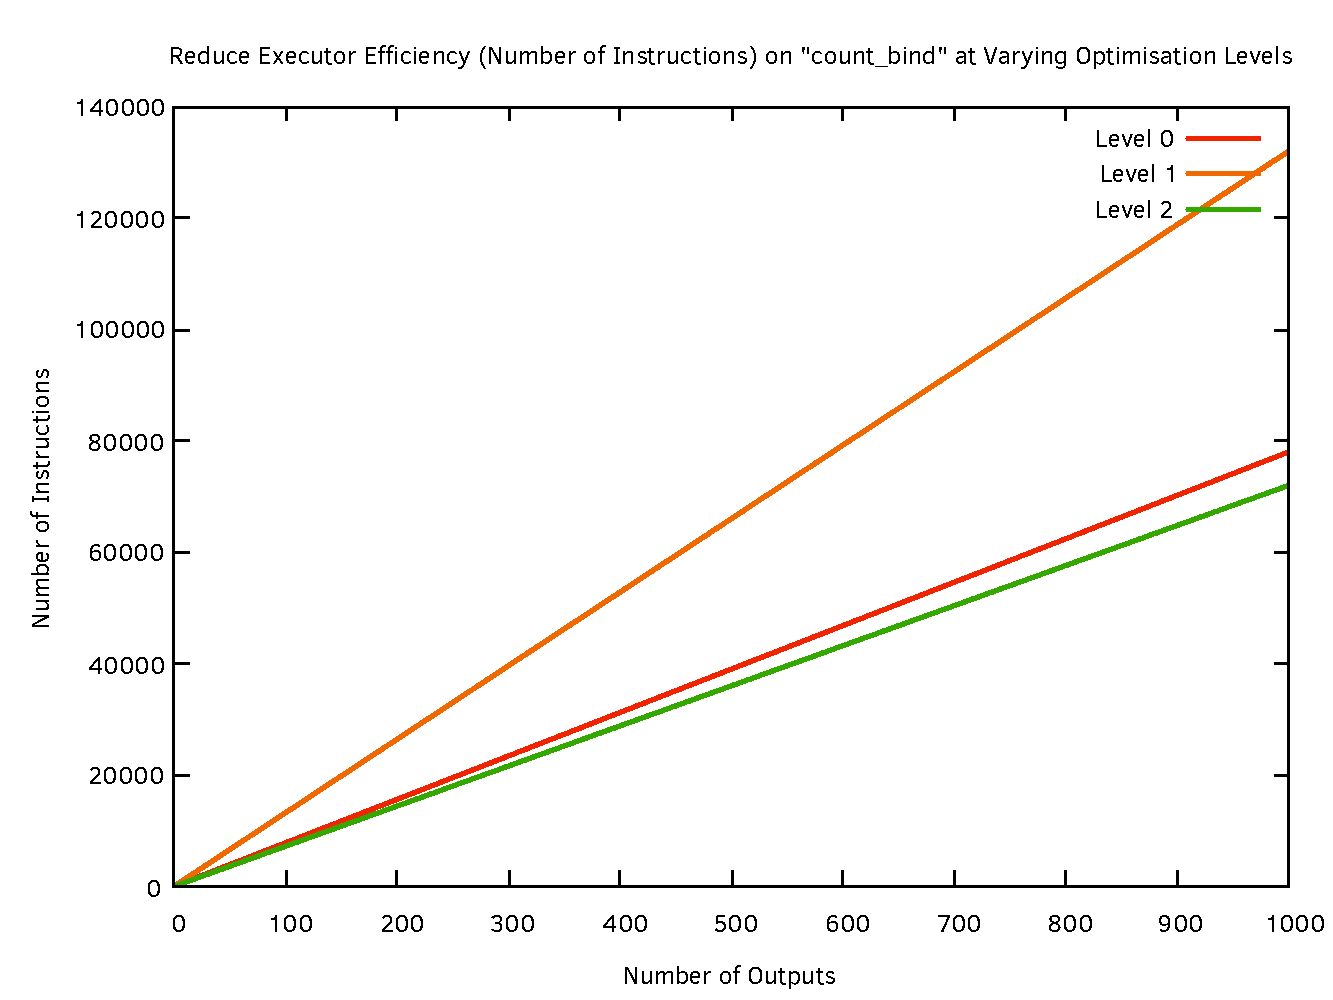
\includegraphics[width=\textwidth - 60pt]{04_results/images/reduce_count_bind_efficiency}
    \caption{Reduce Executor Efficiency on Count\_Bind at varying optimisation levels}
    \label{fig:reduce_count_bind_efficiency}
\end{figure}
\begin{figure}[htb]
    \centering
    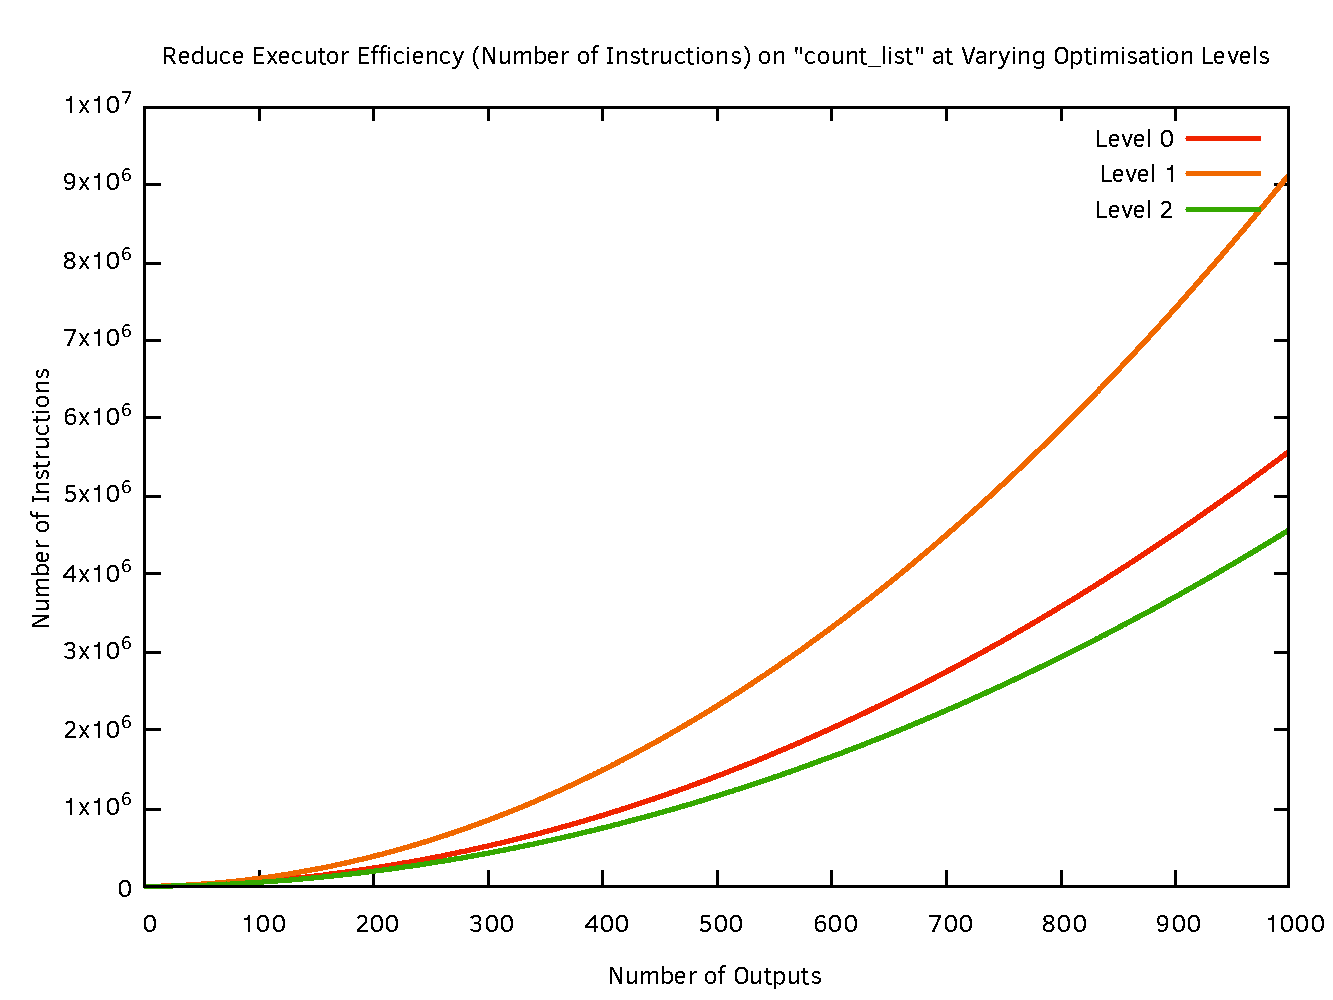
\includegraphics[width=\textwidth - 60pt]{04_results/images/reduce_count_list_efficiency}
    \caption{Reduce Executor Efficiency on Count\_List at varying optimisation levels}
    \label{fig:reduce_count_list_efficiency}
\end{figure}


